%%%%%%%%%%%%%%%%%%%%%%%%%%%%%%%%%%%%%%%%%
% fphw Assignment
% LaTeX Template
% Version 1.0 (27/04/2019)
%
% This template originates from:
% https://www.LaTeXTemplates.com
%
% Authors:
% Class by Felipe Portales-Oliva (f.portales.oliva@gmail.com) with template 
% content and modifications by Vel (vel@LaTeXTemplates.com)
%
% Template (this file) License:
% CC BY-NC-SA 3.0 (http://creativecommons.org/licenses/by-nc-sa/3.0/)
%
%%%%%%%%%%%%%%%%%%%%%%%%%%%%%%%%%%%%%%%%%

%----------------------------------------------------------------------------------------
%	PACKAGES AND OTHER DOCUMENT CONFIGURATIONS
%----------------------------------------------------------------------------------------

\documentclass[
	12pt, % Default font size, values between 10pt-12pt are allowed
	%letterpaper, % Uncomment for US letter paper size
	%spanish, % Uncomment for Spanish
]{fphw}

% Template-specific packages
\usepackage[utf8]{inputenc} % Required for inputting international characters
\usepackage[T1]{fontenc} % Output font encoding for international characters
\usepackage{mathpazo} % Use the Palatino font
\usepackage[dvipsnames]{xcolor}
\usepackage{graphicx} % Required for including images
\usepackage{amsmath}
\usepackage{booktabs} % Required for better horizontal rules in tables
\usepackage{listings} % Required for insertion of code
\usepackage{enumerate} % To modify the enumerate environment
\usepackage{ragged2e}
\usepackage{cancel}
\usepackage{MnSymbol,bbding,pifont}
\usepackage{lscape}
\usepackage{array}
\usepackage{float,graphicx}
\newcolumntype{M}{>{$}c<{$}}
%----------------------------------------------------------------------------------------
%	ASSIGNMENT INFORMATION
%----------------------------------------------------------------------------------------

\title{Assignment \#3} % Assignment title

\author{Luis Alberto Ballado Aradias} % Student name

\date{\today} % Due date

\institute{Centro de Investigación y de Estudios Avanzados del IPN \\ Unidad Tamaulipas} % Institute or school name

\class{Tecnologías Computacionales (Sep - Dec 2022)} % Course or class name

\professor{Dr. Edwin Aldana Bobadilla} % Professor or teacher in charge of the assignment

%----------------------------------------------------------------------------------------

\begin{document}

\maketitle % Output the assignment title, created automatically using the information in the custom commands above

%----------------------------------------------------------------------------------------
%	ASSIGNMENT CONTENT
%----------------------------------------------------------------------------------------
{\color{teal}
\dotfill
Chomsky Hierarchy
\dotfill}

Any language is a structured medium of communication no matter if it is spoken or written natural language, coded or sign language, or a formal programming language such as Python or Java. Languages are characterised by two basic elements: \textbf{syntax} (grammatical rules) and \textbf{semantics} (meaning). In language like the way we communicate each other, the meaning might vary depending upon a third factor \textbf{context of usage}.\\

Depending on restrictions and complexity present in the grammar, languages find a place in the hierarchy of formal languages. \textbf{Noam Chomsky}, an American linguist cum cognitive scientist, defined this hierarchy in 1956 and hence it is calles \textbf{Chomsky Hierarchy}.\\

Although his concept is quite old, there is renewed interest because of it is relevance to Natural Language Processing. Chomsky Hierarchy help us answer question like \textbf{Can a natural language like Spanish be described .. parsed, or even compiled} with the same methods as used for formal or artificial languages in Computer Science?

\begin{figure}[H]
  \centering
  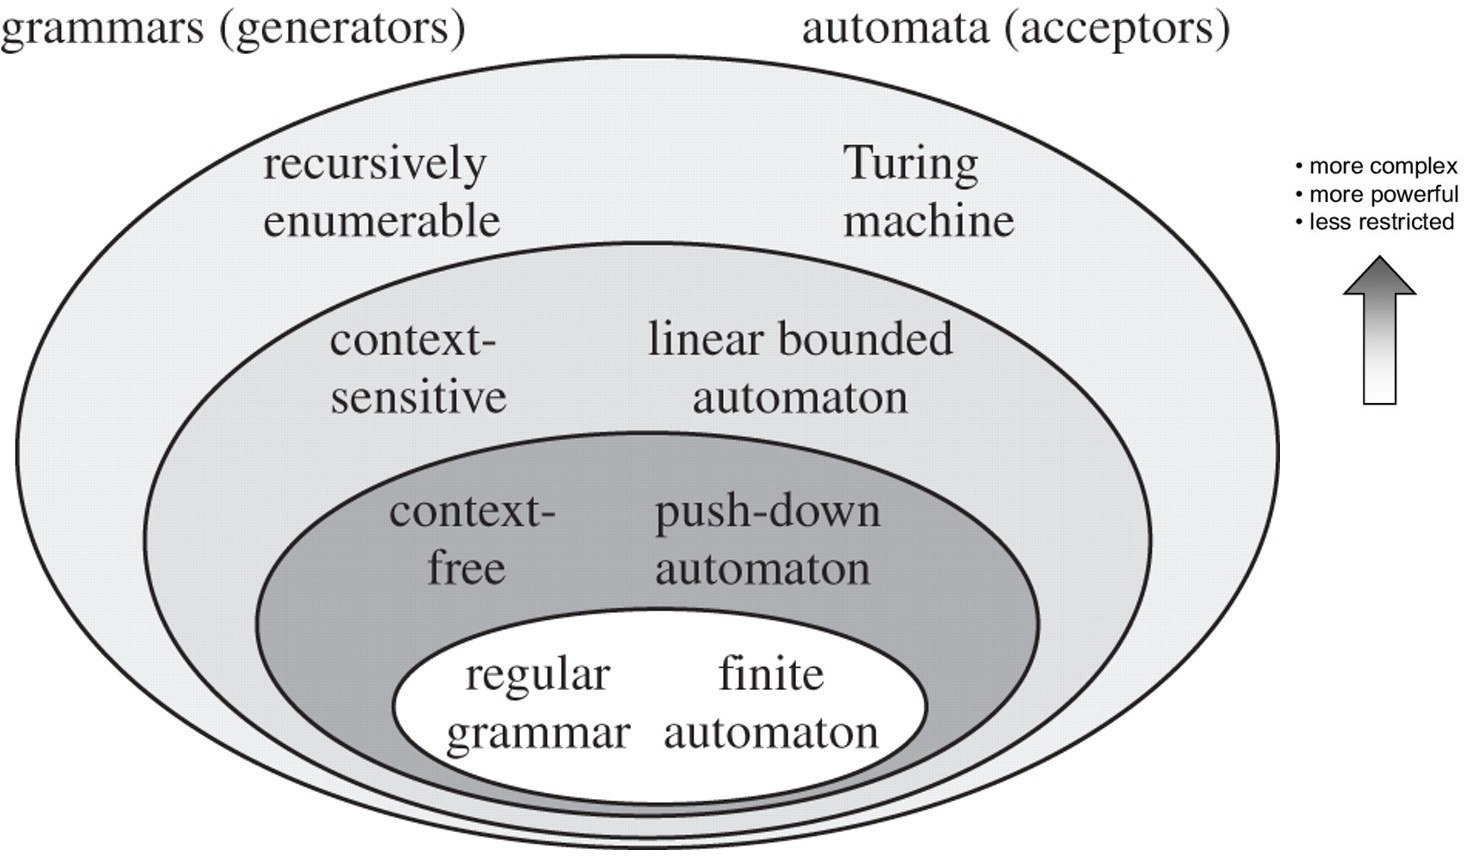
\includegraphics[scale=0.5]{images/chomsky_hierarchy.jpg}
\end{figure}

\newpage
According to Chomsky hierarchy, grammar is divided into 4 types:
\begin{enumerate}
\item Regular Grammar
\item Context Free Grammar (deterministic and non deterministic)
\item Context Sesitive Grammar  
\item Recursively-enumerable Grammar
\end{enumerate}

\section*{{\color{BlueViolet}Regular Grammar}}

Most restrictive of the set, they generate regular languages. They must have a single non-terminal on the left-hand-side and a right-hand-side consisting of a single terminal or single terminal followed by a single non-terminal.\\\\

\textbf{Example:}\\

Regex to define tokens such as identifiers, language keywords in programming languages. A coin vending machine that accepts only 1-Rupee, 2-Rupee and 5-Rupee coins has a regular language with only three words – 1, 2, 5.


\section*{{\color{Apricot}Context-Free Grammar}}
%------------------------------------------------

Generate context-free languages, a category of immense interest to NLP practitioners. Here all rules take the form $A \implies \beta$, where A is a single non-terminal symbol and $\beta$ is a string of symbols.\\\\

\textbf{Example:}\\

Statement blocks in programming languages such as functions in parentheses, If-Else, for loops. In natural language, nouns and their plurals can be recognized through one Non Deterministic Finite Automaton (NFA), verbs and their different forms can be recognized through another NFA, and then combined. \\Singular (The girl runs home $\implies$ Girl + Runs). \\Plural (The girls run home $\implies$ Girls + Run)

%----------------------------------------------------------------------------------------

\section*{{\color{Cerulean}Context-Sensitive Grammar}}
%------------------------------------------------
The highest programmable level, they generate context-sensitive languages. They have rules of the form $\alpha A \beta \implies \alpha \gamma \beta$ with A as a non-terminal and $\alpha$, $\beta$, $\gamma$ as strings of terminals and non-terminals. Strings $\alpha$, $\beta$ may be empty, but $\gamma$ must be nonempty.\\\\

\textbf{Example:}\\

Though most language constructs in natural language are context-free, in some situations linear matching of tokens has to be done, such as - The square roots of 16, 9 and 4 are 4, 3 and 2, respectively. Here 16 is to be matched with 4, 9 is matched with 3, and 4 is matched with 2.

\section*{{\color{RoyalPurple}Recursively enumerable grammar}}
%------------------------------------------------
Are too generic and unrestricted to describe the syntax of either programming or natural languages\\\\

\textbf{Example:}\\

A language with no restrictions is not conducive to communication or automation. Hence there are no common examples for this type. However, some mathematical seemingly unsolvable equations are expressed in this form.

%----------------------------------------------------------------------------------------

\newpage
\section*{{\color{RoyalPurple}Regular Expression in Real Application}}

Exercise: Create a regular expression to accept vehicle registration plates of Mexico State. There are three-letter series assigned \textbf{LGA-PEZ}

\begin{figure}[H]
  \centering
  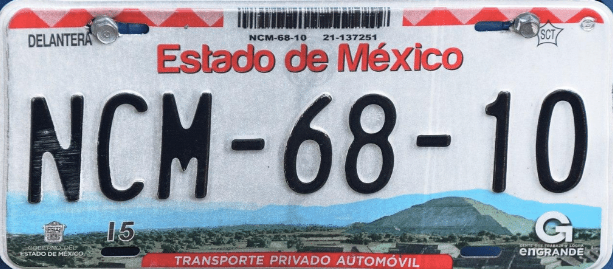
\includegraphics[scale=0.4]{images/placa_auto.png}
\end{figure}

\begin{verbatim}
/^[L-P]{1}[G-ZA-E]{1}[A-Z]{1}-\d{2}-\d{2}$/
\end{verbatim}

Explanation:\\

\begin{itemize}
\item  $\wedge$ asserts position at start of the string
\item Match a single character present in the list below $\boldsymbol{[L-P]\{1\}}$ matches the previous token exactly \textbf{one} time (meaningless quantifier)\\
  $\boldsymbol{[L-P]}$ matches a single character in the range between L and P (case sensitive)
\item Match a single character present in the list below $\boldsymbol{[G-ZA-E]\{1\}}$ matches the previous token exactly \textbf{one} time (meaningless quantifier)\\
  $\boldsymbol{[G-Z]}$ matches a single character in the range between G and Z (case sensitive)\\
\item Match a single character present in the list below $\boldsymbol{[A-Z]\{1\}}$ matches the previous token exactly one time (meaningless quantifier)\\
  $\boldsymbol{[A-Z]}$ matches a single character in the range between A and Z (case sensitive)
\item $\boldsymbol{\textbackslash d}$ matches a digit (equivalent to [0-9])\\
  $\boldsymbol{\{2\}}$ matches the previous token exactly 2 times
\item $\boldsymbol{\textbackslash d}$ matches a digit (equivalent to [0-9])\\
  $\boldsymbol{\{2\}}$ matches the previous token exactly 2 times
  \item $\boldsymbol{\$}$ asserts position at the end of the string, or before the line terminator right at the end of the string (if any)
\end{itemize}

\end{document}
